\section{Follow-up study (v2): an improved circuit, re-tested on fresh seeds}
\label{sec:followup}

The diagnostics of \S\ref{sec:diagnostics} point to a specific change: give the output
layer independent handles on the circuit's Fourier amplitudes. Testing it honestly
needs the same discipline as v1: tune on old data, commit predictions, then test on
runs that did not exist when the predictions were written.

\paragraph{Design} (\texttt{docs/superpowers/specs/2026-09-28-*-design.md}, committed
before any run). The v2 model keeps SMCD's circuit and adds $K$ copies of it (same
encoding scalings, hence the same $\Omega$; each with its own angles) mixed by a linear
head. Every classical family received the same number of tuning configurations as the
quantum model. Tuning used only v1's Poisson problem with seeds 0--2, and the selection
rule, including a parsimony rule on $K$, was committed before the first lab result
(\texttt{scripts/select\_v2\_config.py}). A planned second tuning arm (the affine
boundary ansatz) was stopped before it ran, under the paper deadline (design spec,
amendment 5), which also restricted the re-test to the Poisson claims and the
groundwater problem.

\paragraph{The lab} (tuning seeds; exploratory). Eight copies at learning rate
$10^{-2}$ (91 parameters) reached a median rel-$L^2$ of 0.003 on Poisson, against 1.67
for v1's circuit, 0.27 for \texttt{c\_rff\_matched} (13 parameters), 0.19 for
\texttt{c\_ff} (129) and 0.0004 for \texttt{c\_mlp} (8{,}513)
(Figure~\ref{fig:v2lab}). This configuration was selected by the committed rule, and
its lab number was seen before the re-test predictions were written
(\texttt{docs/predictions\_v2.md} says so).

\paragraph{The re-test} (seeds 10--14, pushed to GitHub before any run;
\texttt{scripts/verify\_preregistration.py --v2}: 31 runs checked, 0 violations).
v1's claims were re-adjudicated word for word by the unchanged script
(Table~\ref{tab:v2}, Figure~\ref{fig:v2retest}). \textbf{Of the eight re-tested
claims, five held.} The v2 circuit's median error is 0.0037 with every seed below
0.02. It beats \texttt{c\_ff} (R-2) and the same circuit with random frequencies by
236$\times$ (R-6); 99.9\% of its improvement over \texttt{c\_mlp} lies inside $\Omega$
(R-8); its encoder drifts by 0.10 (R-12); and with 91 parameters its NTK has
eigenvalues beyond index $|\Omega|=81$, so R-7 becomes measurable, and the spectrum is
flatter inside $\Omega$ than outside by 15.2 (the bar is 0.5).

Three results temper this. First, \textbf{a classical model with the same frequencies
and nearly the same size (83 parameters) is still 3.3$\times$ more accurate} (median
0.0011; R-3 predicted parity and is refuted), so the circuit's gain over v1 is a gain
in trainability, not an advantage over the matched classical model. Second, R-1 against
\texttt{c\_mlp} is inconclusive: at its tuned learning rate the MLP failed on three of
five fresh seeds (1.2--3.6) and reached 0.003--0.012 on the other two. Third, the
classical learning rates chosen in the lab did not carry over to fresh seeds
(\texttt{c\_ff} went from a lab median of 0.19 to 5.0), which inflates R-1 and R-2's
ratios; against v1's untuned baselines on seeds 0--4 (\texttt{c\_mlp} 1.08,
\texttt{c\_ff} 0.21) the v2 circuit is still ahead, though those are not paired seeds.
R-11 is refuted as in v1. The claims on heat, Helmholtz and the sweeps (R-4, R-5, R-9,
R-10) were not re-tested in this round.

% Generated by scripts/report/paper_tables.py from results/adjudication_v2.json.
\begin{table}[htbp]
  \centering
  \small
  \begin{tabular}{llr}
  \toprule
  Claim & Verdict & Measured \\
  \midrule
  R-1 & Inconclusive & 337.79$\times$ \\
  R-2 & \textbf{Confirmed} & 1359.81$\times$ \\
  R-3 & Refuted & 3.30$\times$ \\
  R-6 (poisson) & \textbf{Confirmed} & 236.08$\times$ \\
  R-7 (poisson) & \textbf{Confirmed} & gap 15.2 \\
  R-8 (poisson) & \textbf{Confirmed} & 99.9\% in $\Omega$ \\
  R-11 & Refuted &  \\
  R-12 & \textbf{Confirmed} & drift 0.10 \\
  \bottomrule
  \end{tabular}
  \caption{v1's claims re-tested on the v2 model, seeds 10--14 (Poisson). Ratios as each
    claim defines them: R-1, R-2 and R-6 give baseline error over v2 error (above 1: v2 better);
    R-3 gives v2 error over \texttt{c\_rff\_matched\_v2} error (3.3: v2 worse). Claims on other
    problems were not run in this round.}
  \label{tab:v2}
\end{table}


\begin{figure}[htbp]
  \centering
  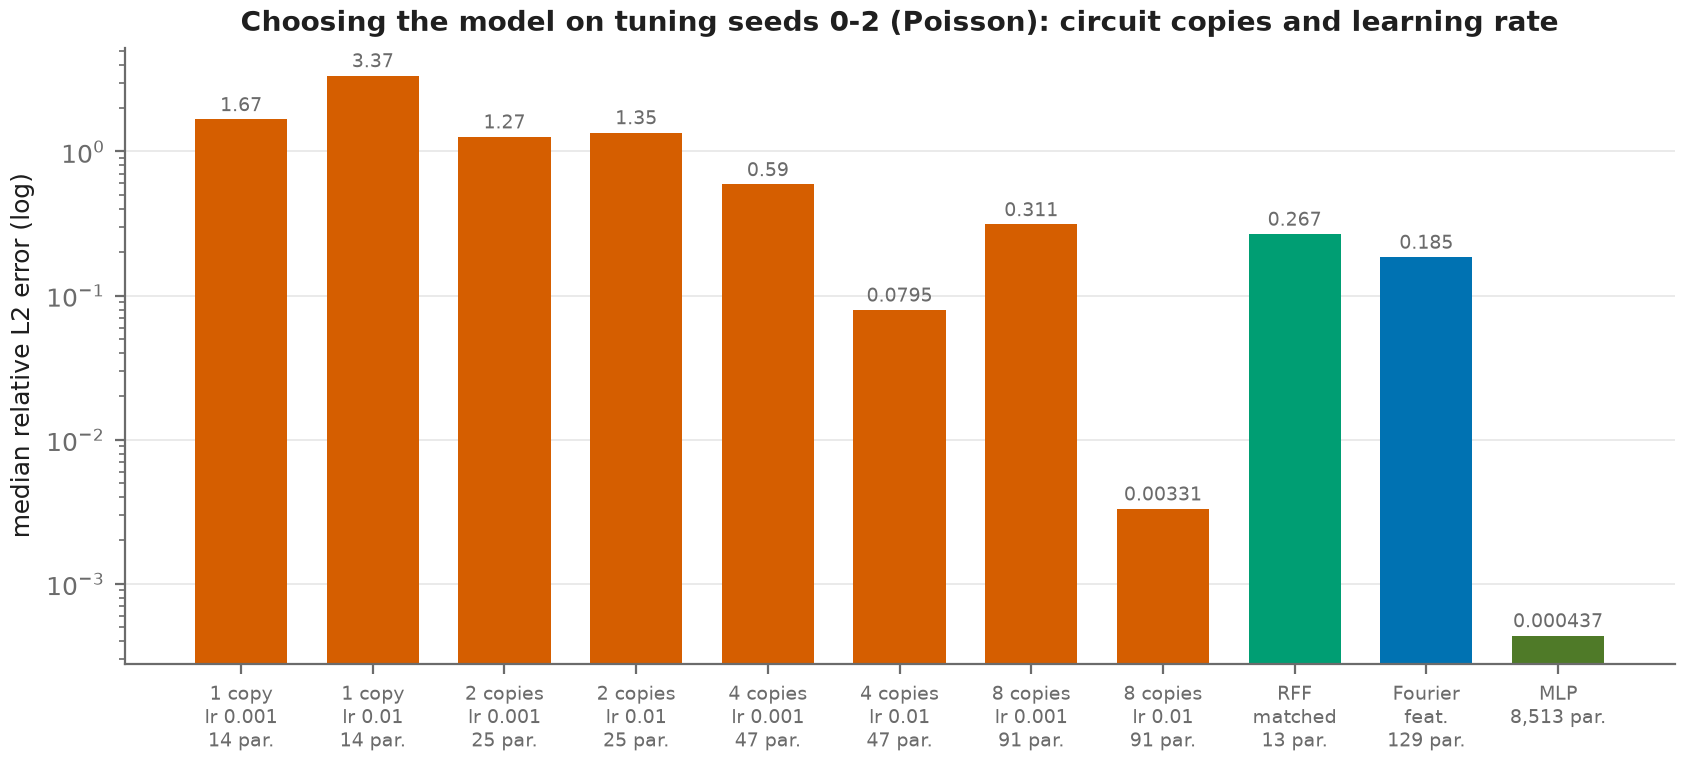
\includegraphics[width=\linewidth]{../results/report/figures/headline_v2_lab.png}
  \caption{The v2 lab on Poisson, tuning seeds 0--2 (exploratory): median error of each
    quantum configuration and of the best learning rate for each classical model.}
  \label{fig:v2lab}
\end{figure}

\begin{figure}[htbp]
  \centering
  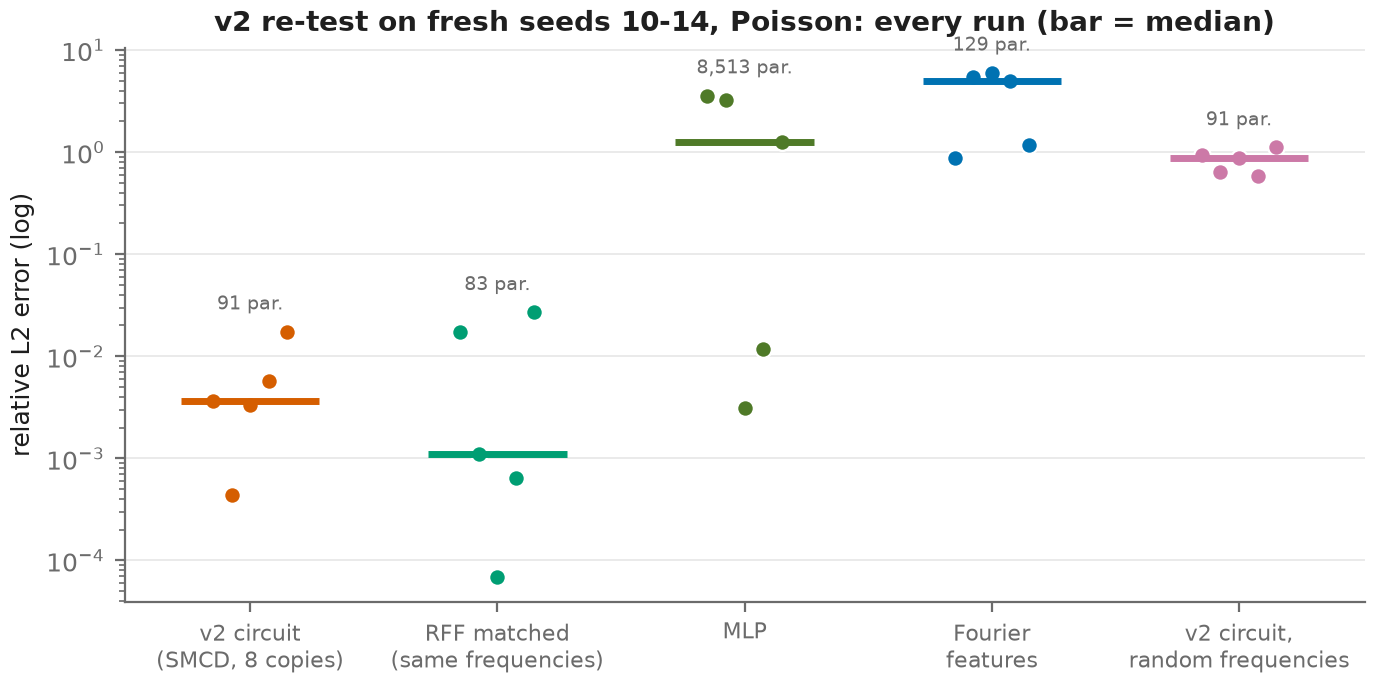
\includegraphics[width=0.9\linewidth]{../results/report/figures/headline_v2_retest.png}
  \caption{The pre-registered v2 re-test on Poisson: every run on fresh seeds 10--14.}
  \label{fig:v2retest}
\end{figure}
